The chosen model system of five inhibitors of CHK1 kinase exemplifies different core-hopping transformations (i.e. ring size change, ring opening/closing, ring extension) and R-group modifications \cite{Wang2017}, increasing the complexity compared to the systems previously studied with RE-EDS. Furthermore, the performance can be directly compared to the results obtained with FEP+ and OPLS3 in Ref.~\cite{Wang2017} as well as with QligFEP results in Ref.~\cite{Jespers2019}.

\subsection{Parameter Exploration and Parameter Optimization}
The RE-EDS workflow was started by estimating the lower bound for the $s$-distribution. Using the above mentioned undersampling criterion (see Methods section), a lower bound of $s=0.003$ was determined. 
%State Optimizations
Optimized coordinates were obtained for all five ligands, as verified by comparing the potential-energy distribution from the EDS simulation with the one extracted from a standard MD simulation of the respective ligand (Figure S1 in the Supporting Information). % SUPPL
From these same steps, the potential-energy thresholds for the occurrence sampling ($T_{i}^{\text{phys}}$) and undersampling ($T_{i}^{\text{us}}$) were estimated.

%Eoff:
The energy offsets $\vec{E}^R$ were estimated from a short RE-EDS simulation with the PEOE \cite{Sidler2016} scheme and are listed in Table \ref{tab:CHK1_set2_Eoff}.
For $s=1.0$, the energy offsets should ideally be equal to the free energy of the corresponding state (i.e. $\Delta E^R_{ji} = \Delta G_{ji}$) such that the partition function of the reference state is the sum of the partition functions of the end states \cite{Christ2008}. Therefore, the comparison between the relative estimated energy offsets in water and in complex ($\Delta \Delta E^R_{ji} = \Delta E^R_{ji,\text{complex}} - \Delta E^R_{ji,\text{water}}$) and the relative binding free energy $\Delta \Delta G^\text{bind}_{ji}$ can be used to (roughly) assess the quality of the estimated energy offsets. As shown in Figure S2 in the Supporting Information, % SUPPL
the energy offsets estimated from the SSM simulations are in better agreement with the experimental relative binding free energies than those estimated from the 1SS simulations.

\begin{table}[h]
	\caption{Energy offsets $\vec{E^R}$ estimated from a short RE-EDS simulation using the PEOE \cite{Sidler2016} scheme. The errors indicate the standard deviation over the different replicas in undersampling. All energy offsets were calculated relative to ligand L1. The starting coordinates were selected following the 1SS or the SSM approach (see Theory and Methods sections).}
	\label{tab:CHK1_set2_Eoff}
	\resizebox{\columnwidth}{!}{%
		\centering
		\begin{tabular}{ l | r r | r r }
			Ligand & \multicolumn{2}{c|}{RE-EDS 1SS}&\multicolumn{2}{c}{RE-EDS SSM}  \\ 
			&Water [kJ~mol$^{-1}$]&Complex [kJ~mol$^{-1}$]&Water [kJ~mol$^{-1}$]&Complex [kJ~mol$^{-1}$]\\ 
			\hline
			L1 & $0.0$ & $0.0$ & $0.0$ & $0.0$ \\ 
			L17 & $15.9 \pm 4.9 $ & $14.1 \pm 1.9 $ & $12.9 \pm 2.3 $ & $19.1 \pm 3.2$ \\
			L19 & $9.6 \pm 5.3 $ & $ -5.8 \pm 0.5 $ & $-5.4 \pm 4.7 $ & $ -2.3 \pm 3.1$ \\
			L20 & $-52.4 \pm 4.4$ & $ -48.5 \pm 3.0$ & $ -49.7 \pm 8.8 $ & $-55.0 \pm 1.5$\\
			L21 & $-69.9 \pm 1.8 $&$ -70.0 \pm 8.8$ & $ -72.5 \pm 6.0 $ & $ -72.9 \pm 3.0$\\
		\end{tabular}
	}
\end{table}

%S-Optimization
The optimization of the $s$-distribution was performed with the N-LRTO \cite{Sidler2017} algorithm, thereby minimizing the average round-trip time $\overline{\tau}$ in the replica graph. 
%
In the first iteration, the number of total round trips is relatively small and the average round-trip time is large for all simulations (Figure \ref{fig: CHK1_RingOpening_sOptimization}). The number of round trips is smaller in the complex than in water due to a more pronounced gap region \cite{Sidler2017}.
Already after the second iteration, the round-trip time is generally reduced. An exception was observed for 
RE-EDS 1SS in the complex, where no round trips occurred during the second iteration. The improvement of the $\overline{\tau}$ over the iterations can also be seen in Figure S4 in the Supporting Information. % SUPPL
%% s-replica placements
As can be seen in the third row of Figure \ref{fig: CHK1_RingOpening_sOptimization}, the optimization algorithm increases the density of the replicas around $s = 0.041$, where the major gap region lies.

\begin{figure}[h]
	\centering
	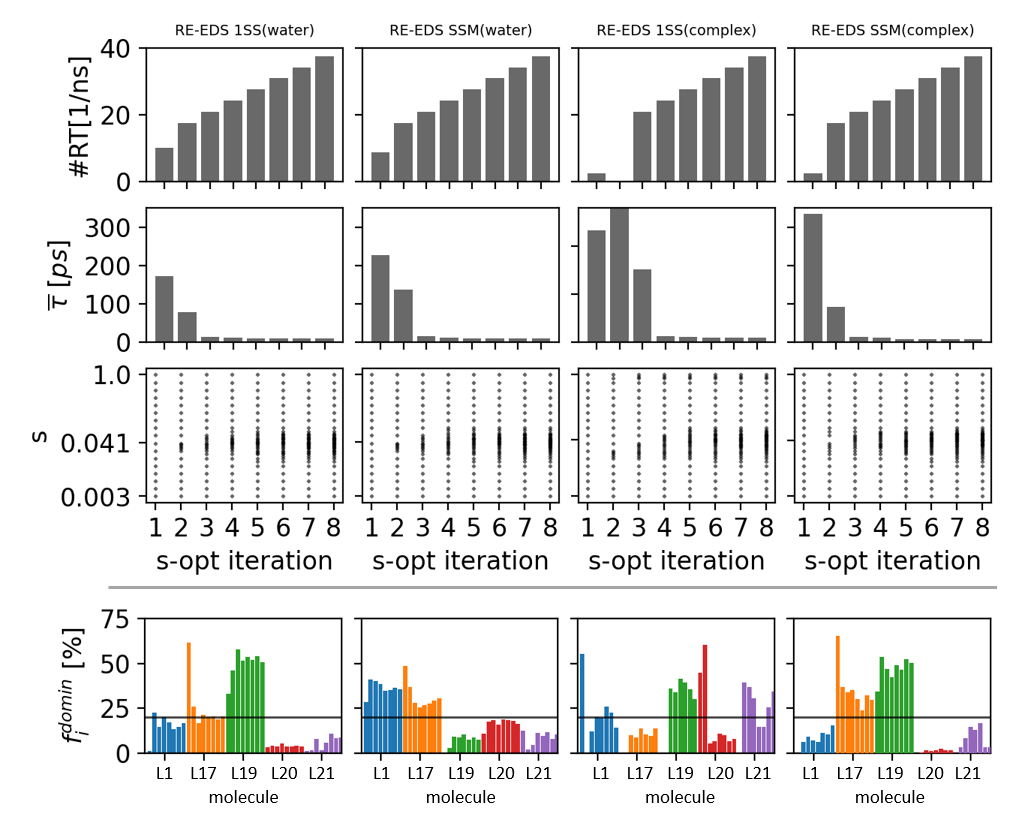
\includegraphics[width=\textwidth]{fig/results/ringOpening/paramOptimization/S-optimization_ringOpening.png}
	\caption{Optimization of the $s$-distribution with the N-LRTO \cite{Sidler2017} algorithm over eight iterations. The measured quality criteria were the number of round trips (1. row), the average round-trip time $\overline{\tau}$ (2. row), the placement of the replicas in $s$-space (3. row), and the sampling fractions of dominating states $f_{i}^{\text{domin}}$ (4. row).}
	\label{fig: CHK1_RingOpening_sOptimization}
\end{figure}

%% states sampling
In addition, we monitored the relative sampling of the end states at $s=1.0$ during the iterations.
Ideally, each end state should be sampled equally in an optimized RE-EDS simulation (see Eq. (\ref{eq: optimalDominationSamplingDist})).  The last row in Figure \ref{fig: CHK1_RingOpening_sOptimization} shows $f_{i}^{\text{domin}}$ as a function of the iteration. For all end states, the sampling fraction converges (slowly) towards the ideal value.
%% tau converge - Conclusion
The $s$-optimization for the ligands in water converged after the fourth iteration with $\Delta \overline{\tau} < 10~ps$ (Figure S4 in the Supporting Information). % SUPPL
This resulted in the final 36 replicas.
For the protein-ligands complex, the optimization converged after the fifth iteration, resulting in 41 replicas. 
The average round-trip time after convergence was $\overline{\tau} = 9.6 \pm 0.9$~ps for all simulations.

\subsection{Free-Energy Calculation}
After successfully optimizing the RE-EDS parameters, the production runs were performed for $4$~ns. 
%%Sampling++
Both in water and in complex, the potential-energy distributions of the end states match generally well the corresponding distributions from the standard MD simulations of the single end states (Figure \ref{fig:RingOpening_sampling_comparison}). 
%
The analysis of the dominating end states at $s=1.0$ shows that L19 is generally oversampled, while L20 and/or L21 are less sampled than expected (Figure S5 in the Supporting Information). % SUPPL
At $s=1.0$, $f_i^{\text{occur}}$ and $f_i^{\text{domin}}$ are very similar, which indicates sampling of clearly separated states in those simulations.

\begin{figure}[h]
	\centering
	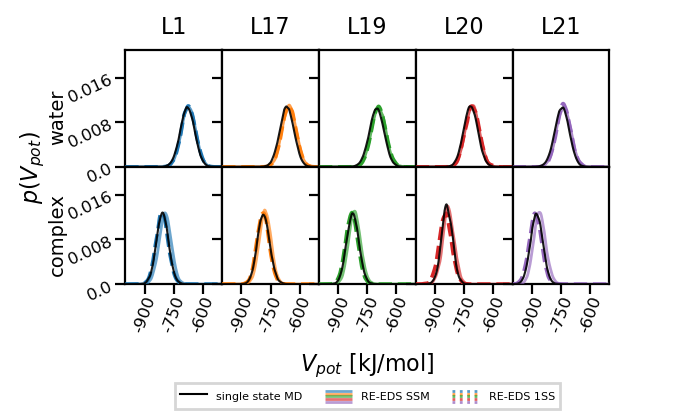
\includegraphics[width=\columnwidth]{fig/results/ringOpening/FE/RingClosure_system_final_sampling.png}
	\caption{Comparison of the Boltzmann reweighted potential-energy distributions obtained from standard MD simulations of a given end state (black) and from the RE-EDS production runs (colored).}
	\label{fig:RingOpening_sampling_comparison}
\end{figure}

%%Accuracy
From the replica at $s=1.0$, the free-energy differences were calculated using Eq.~(\ref{EQ: Free Energy calculation via reference state}) and the resulting $\Delta \Delta G^\text{bind}_{ji}$ were compared with the experimental results taken from Ref.~\cite{Huang2012}. The results are shown graphically in Figure \ref{fig:CHK1_set2_FreeEnergyCalculation} and numerically in Table \ref{SItab: RE-EDS_FE_RingCycleOpening_ddF}. The individual free-energy differences are given in Table S3 in the Supporting Information. %SUPPL
The RMSE with RE-EDS 1SS is $7.3$~kJ~mol$^{-1}$ and the MAE is $5.75\pm4.4$~kJ~mol$^{-1}$. 
%
%how I calculate the MAE and RMSD:
%MAE = np.mean(np.abs(ddG_differences))
%std(MAE) = np.std(np.abs(ddG_differences)) #gives an impression of absolute deviation of all ddG_diffs
%RMSE = np.sqrt(np.mean(np.square(ddG_differences))
%
The main deviations stem from ligand L19 in the RE-EDS 1SS approach.

The performance was substantially improved using the SSM approach with RE-EDS, giving an RMSE of $2.5$~kJ~mol$^{-1}$ and an MAE of $2.1 \pm 1.3$~kJ~mol$^{-1}$. 
Only one value (L21-L17) deviates more than $4.184$~kJ~mol$^{-1}$ (i.e. $1$~kcal~mol$^{-1}$) from experiment.
The Spearman correlation coefficient for RE-EDS 1SS is $r^2_{\text{Spearman}}=0.87$ and for RE-EDS SSM $r^2_{\text{Spearman}}=0.84$.

%%Performance:
Next, we assessed the convergence of the $\Delta G_{ji}$ values as a function of simulation time (Figure S7 in the Supporting Information). % SUPPL
For the RE-EDS 1SS approach, all free-energy differences appeared converged after $1.48$~ns in water and after $1.04$~ns in the complex. For the RE-EDS SSM approach, convergence was observed after $0.52$~ns in water and after $0.88$~ns in the complex. These findings indicate that the use of different starting configurations representing all end states enhances sampling further and reduces the simulation time needed to obtain converged results.

\begin{figure}[h]
	\centering
	\begin{subfigure}{0.85\columnwidth}
		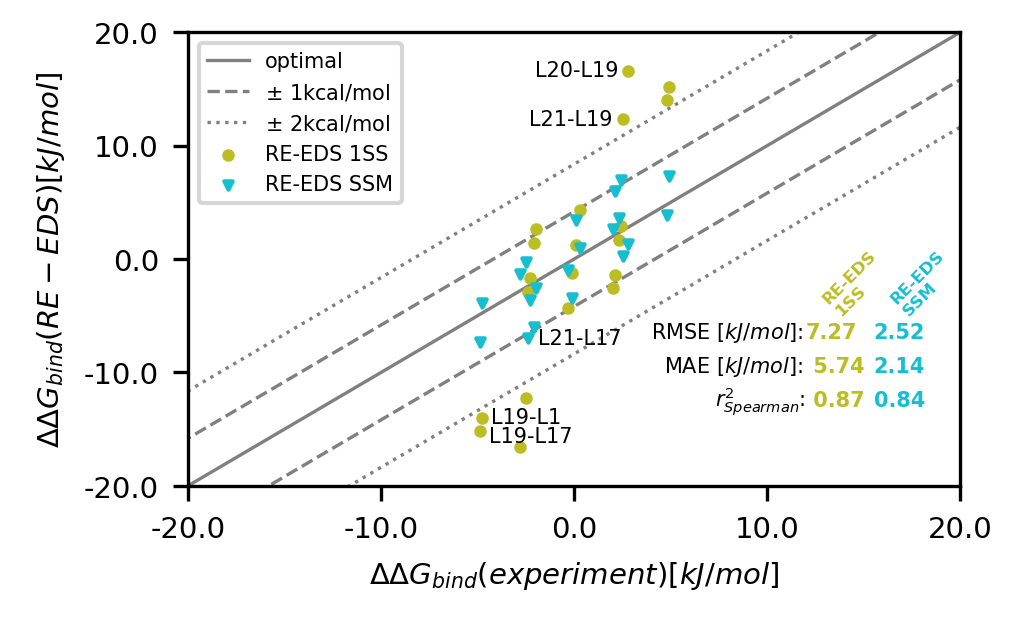
\includegraphics[width=\textwidth]{fig/results/ringOpening/FE/RingClosure_system_final_results_4ns.png}
	\end{subfigure}
	\begin{subfigure}{0.85\columnwidth}
		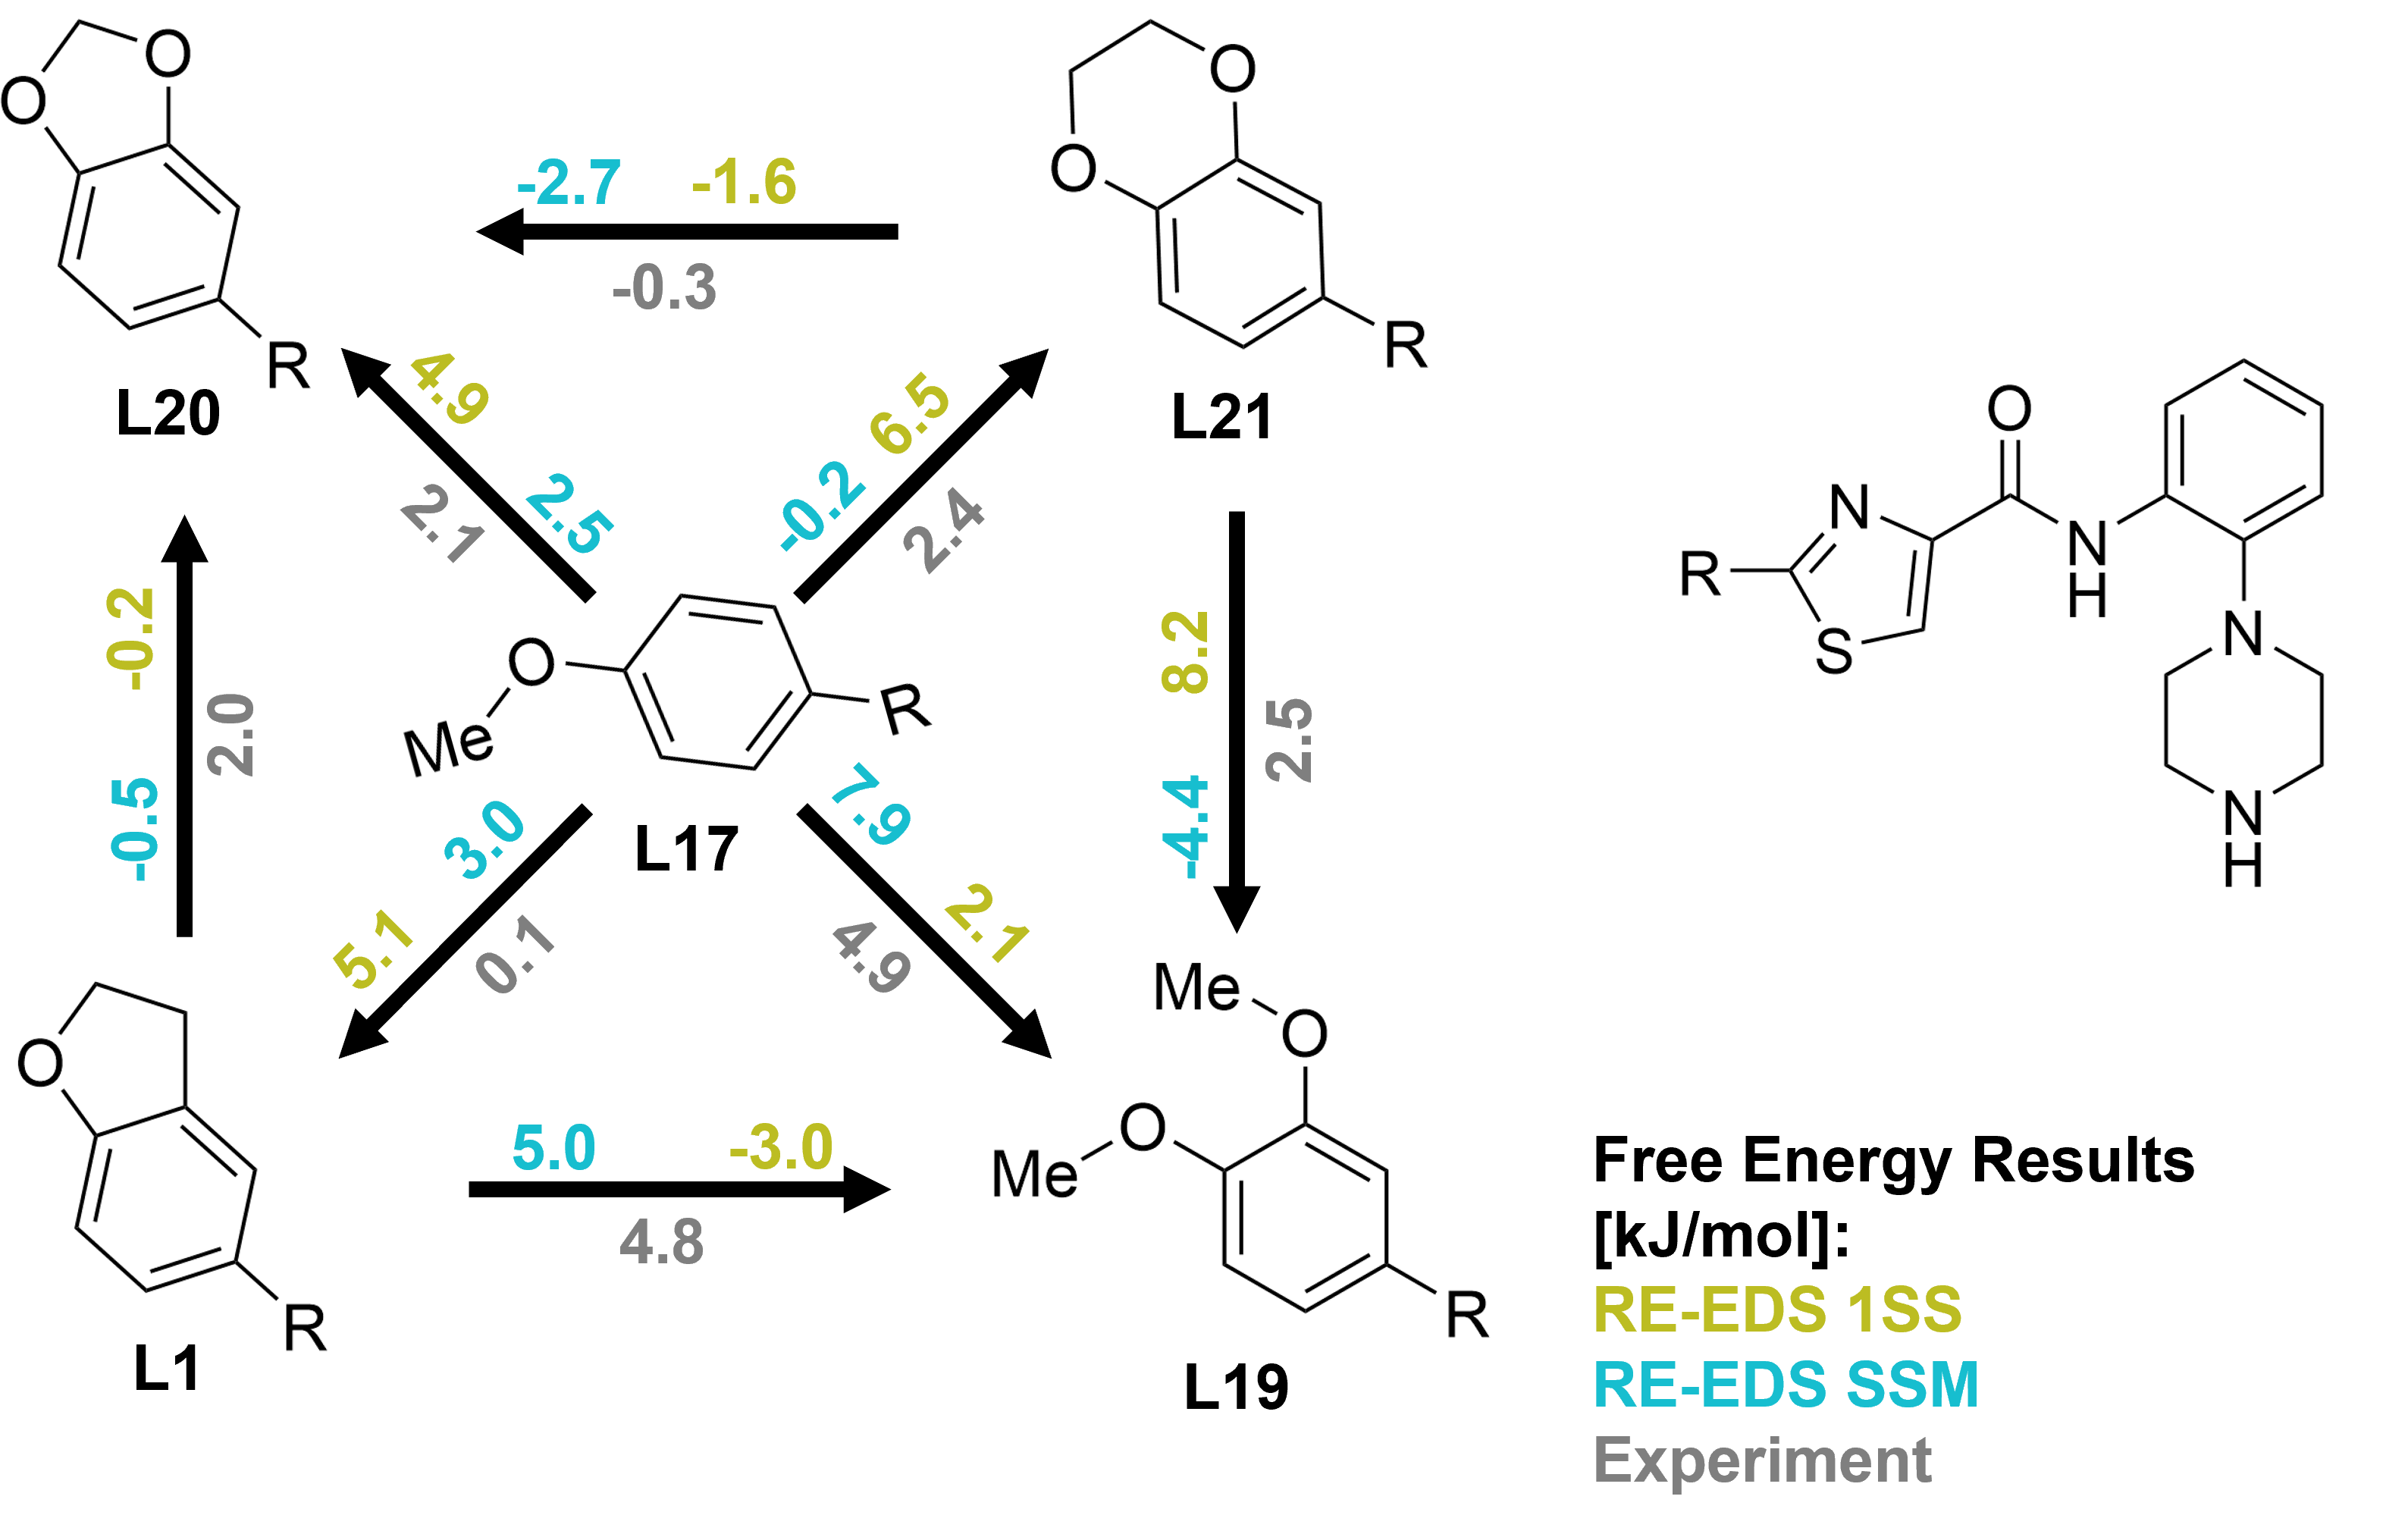
\includegraphics[width=\textwidth]{fig/results/ringOpening/FE/ddG_bind_paper_comparison_reeds_only_4nsSimulation.png}
	\end{subfigure}
	\caption{Free-energy differences estimated from the production run of $4$~ns length. (Top): Comparison between the experimental and calculated $\Delta \Delta G^\text{bind}_{ji}$ using RE-EDS 1SS and RE-EDS SSM. (Bottom): Graphical representation of the $\Delta \Delta G^\text{bind}_{ji}$ results with structures, inspired by the one in Ref.~\cite{Wang2017}.}
	\label{fig:CHK1_set2_FreeEnergyCalculation}
\end{figure}

%Comparison results with Schroedinger & Jespers
By applying the RE-EDS methodology to the same system of five CHK1 inhibitors as studied by Wang \textit{et. al.} \cite{Wang2017} and later on also Jespers \textit{et al.} \cite{Jespers2019}, a direct comparison with FEP+ and QligFEP is possible (Table \ref{SItab: RE-EDS_FE_RingCycleOpening_ddF}). Note that the quality metrics were calculated over all possible pairs of ligands, not only those directly calculated by FEP+ and QligFEP.
For FEP+, we obtained an RMSE of $2.4$~kJ~mol$^{-1}$ and an MAE of $1.8 \pm 1.2$~kJ~mol$^{-1}$ with a Spearman correlation coefficient of $r^2_{\text{Spearman}}=0.67$.
Including cycle closure correction (CC) \cite{Wang2017} reduced the RMSE to $2.1$~kJ~mol$^{-1}$ and the MAE to $1.9 \pm 1.0$~kJ~mol$^{-1}$. The Spearman correlation coefficient increased to $r^2_{\text{Spearman}}=0.73$.
Jespers \textit{et al.} \cite{Jespers2019} reported free-energy differences with QligFEP as an average over ten independent replicas, each with significantly less simulation time per $\lambda$-window than in Ref.~\cite{Wang2017}. For QligFEP, an RMSE of $2.3$~kJ~mol$^{-1}$, an MAE of $2.0 \pm 1.2$~kJ~mol$^{-1}$, and a Spearman coefficient of $r^2_{\text{Spearman}}=0.61$ was obtained.

Overall, the performance of RE-EDS SSM is comparable with the pairwise methods. The results with FEP+ CC and QligFEP showed a slightly higher accuracy compared to experiment, likely due to the different force fields used. The Spearman correlation coefficient is higher for both RE-EDS approaches than with the pairwise approaches, indicating a good ranking of the ligands with the RE-EDS method.
A strong correlation with experiment is of interest in drug design approaches, as the ranking of ligands in virtual screening is important to suggest the most promising drug candidates to be synthesized.

In terms of computational cost, the RE-EDS approach (with 4~ns per replica) resulted in about half the total simulation time (in ns) than reported for the FEP+ calculations in Ref.~\cite{Wang2017}. A major advantage of the simultaneous simulation of multiple ligands in a single RE-EDS simulation is that all $N(N-1)/2$ transformations are sampled directly, leading to low statistical errors and removing the need of a state graph. This advantage increases with increasing number of ligands. The current workflow of RE-EDS uses a relatively large amount of simulation time for parameter optimization. Future work will focus on further optimization of the workflow to reduce the pre-processing time. 

\begin{table}[h]
	\caption{Relative binding free energies $\Delta \Delta G^\text{bind}_{ji}$ from experiment and calculated with the RE-EDS 1SS and RE-EDS SSM approaches. For comparison, the results for FEP+ with and without cycle closure (CC) correction taken from Ref.~\cite{Wang2017} and the results for QligFEP taken from Ref.~\cite{Jespers2019} are listed. The free-energy differences of directly simulated paths were used to infer not directly simulated free-energy differences (marked in bold). If multiple indirect paths were possible, their average was used. The errors for QligFEP were determined in Ref.~\cite{Jespers2019} by calculating the standard deviation over ten replicas. For FEP+, the error of the results was taken from the used BAR \cite{Bennett1976} method and the FEP+ CC errors were obtained from the cycle closure analysis. For the RE-EDS approaches, the reported error is based on the statistical uncertainties of the $\Delta G_{ji}^{env}$ values estimated using Gaussian error approximation \cite{Christ2008}.}
	\begin{center}
		\footnotesize
		\resizebox{\columnwidth}{!}{%
			\begin{tabular}{ c c |c |c|c|c|c|c}
				\multicolumn{2}{c|}{Ligands} & \multicolumn{1}{c|}{Exp. \cite{Huang2012}} &\multicolumn{1}{c|}{FEP+ \cite{Wang2017}}&\multicolumn{1}{c|}{FEP+ CC \cite{Wang2017}}&\multicolumn{1}{c|}{QligFEP \cite{Jespers2019}}&\multicolumn{1}{c|}{RE-EDS 1SS}&\multicolumn{1}{c}{RE-EDS SSM}\\ 
				$i$ & $j$  & [kJ~mol$^{-1}$]  & [kJ~mol$^{-1}$] & [kJ~mol$^{-1}$] & [kJ~mol$^{-1}$] & [kJ~mol$^{-1}$] & [kJ~mol$^{-1}$]  \\
				\hline
				L17 &  L1 &   0.1 & -3.6 $\pm$ 0.4          & -2.9 $\pm$ 1.0         & -1.6 $\pm$ 1.7                                     &   1.2 $\pm$ 0.3 &  3.4 $\pm$ 0.2 \\
				L19 &  L1 &  -4.8 & -3.9 $\pm$ 0.3          & -4.0 $\pm$ 0.6         & -1.7 $\pm$ 2.0                                     & -14.0 $\pm$ 0.3 & -3.9 $\pm$ 0.3 \\
				L20 &  L1 &  -2.0 & -2.5 $\pm$ 0.1          & -3.1 $\pm$ 1.0         & -1.3 $\pm$ 1.3                                     &   2.6 $\pm$ 0.3 & -2.6 $\pm$ 0.4 \\
				L21 &  L1 &  -2.3 &\textbf{-3.4} $\pm$ \textbf{0.7}  &\textbf{-3.2} $\pm$ \textbf{1.3} & \textbf{-0.1} $\pm$ \textbf{3.5} &  -1.7 $\pm$ 0.4 & -3.6 $\pm$ 0.9 \\
				L19 &  L17 & -4.9 & -1.4 $\pm$ 0.3          & -1.1 $\pm$ 1.0         & \textbf{0.1} $\pm$ \textbf{2.6}                    & -15.2 $\pm$ 0.2 & -7.3 $\pm$ 0.2 \\
				L20 &  L17 & -2.1 &  0.3 $\pm$ 0.4          & -0.1 $\pm$ 0.8         & -1.3 $\pm$ 2.3                                     &   1.4 $\pm$ 0.3 & -6.0 $\pm$ 0.4 \\
				L21 &  L17 & -2.4 & -1.1 $\pm$ 0.4          & -0.9 $\pm$ 0.9         &\textbf{0.7} $\pm$ \textbf{2.6}                     &  -2.9 $\pm$ 0.4 & -7.0 $\pm$ 0.9 \\
				L20 &  L19 & 2.8  &\textbf{0.8} $\pm$ \textbf{0.6}   & \textbf{0.1} $\pm$ \textbf{1.3} & \textbf{-0.4} $\pm$ \textbf{3.7} &  16.6 $\pm$ 0.4 &  1.3 $\pm$ 0.4 \\
				L21 &  L19 & 2.5  & -0.1 $\pm$ 0.6         &  0.6 $\pm$ 0.1         &  0.6 $\pm$ 4.9                                      &  12.3 $\pm$ 0.5 &  0.3 $\pm$ 0.9 \\
				L21 &  L20 & -0.3 & -0.3 $\pm$ 0.8         & -0.6 $\pm$ 0.8         &  0.6 $\pm$ 1.1                                    &  -4.3 $\pm$ 0.5 & -1.0 $\pm$ 0.9 \\ 
				\hline
				\multicolumn{2}{c|}{RMSE} &                    & 2.4            & 2.1           &  2.3          & 7.3          & 2.5 \\
				\multicolumn{2}{c|}{MAE} &                     & 1.8 $\pm$ 1.2 & 1.9 $\pm$ 1.0 & 2.0 $\pm$ 1.2 & 5.8 $\pm$4.4 & 2.1 $\pm$ 1.3 \\
				%\multicolumn{2}{c|}{$r^2_{\text{Pearson}}$} & & 0.66            & 0.67          & 0.63          & 0.83          & 0.83 \\
				\multicolumn{2}{c|}{$r^2_{\text{Spearman}}$} & & 0.67           & 0.73          & 0.61          & 0.87          & 0.84 \\
			\end{tabular}
		}
	\end{center}
	\label{SItab: RE-EDS_FE_RingCycleOpening_ddF}
\end{table}

% 
%FEP+: 
%MAE 1.99 +- 1.4
%RMSE 2.43
%r^2 pearson 0.56 	 r^2 spearman 0.56
%
%FEP+ CC: 
%MAE 1.88 +- 1.05
%RMSE 2.15
%r^2 pearson 0.66 	 r^2 spearman 0.71

%QLigFEP
%MAE 1.97 +- 1.2
%RMSE 2.3
%r^2 pearson 0.63 	 r^2 spearman 0.61

%1SS: 
%MAE 5.75 +- 4.45
%RMSE 7.27 +- 7.27
%r^2 pearson 0.83 	 r^2 spearman 0.87

%SSM: 
%MAE 2.11 +- 1.32
%RMSE 2.49 +- 2.49
%r^2 pearson 0.83 	 r^2 spearman 0.84


%ComputationalCost
%FEP: 16 l-windwos*5ns*4 pairs * 2 approaches ==> 640ns
%QligFEP: 10 repetitions * (eq 131ps + 51lams * 10ps sim) * 4 pairs * 2 approaches ==> 51ns
%RE-EDS: 4ns * (41+36) ==> 308ns
%RE-EDS opt: eoff(21*0.8)+sop1(0.4ns*21)+sopt2(0.8ns*25)+sopt3(1.2ns*29)+sopt4(1.2ns*31) | == 234.4ns
%+Complex stop water +sopt5(1.2ns*35) == 42ns
